\begin{figure}[p]
     \caption{Gold clause effect on investment by year}
     \begin{center}
    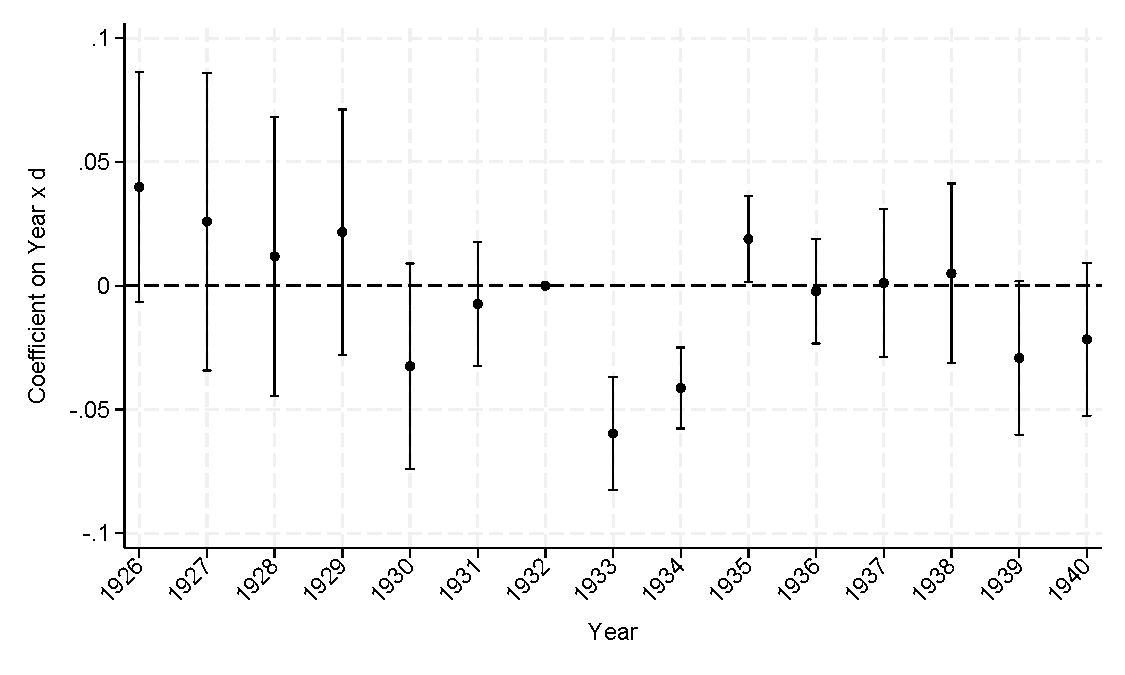
\includegraphics[width=\linewidth]{Figures/gold_coeffs.pdf}
    \end{center}
    \footnotesize \textit{Notes.} This figure plots the point estimates and the 95\% confidence bands from a regression of net investment rate on $Q$ and $d$ interacted with Year including firm and year fixed effects. The estimates are also listed in Column 2 of Table \ref{tab:inv_main}.
    \label{fig:gold_coeffs}
\end{figure}

\begin{table}[p]\centering
\caption{\\ Summary statistics}\scriptsize
\label{tab:sum_main}
  \begin{threeparttable}
\begin{tabular}{lrrrrrrrrr}
\toprule
Variable & Firms & N & Mean & SD & 5\% & 25\% & 50\% & 75\% & 95\% \\
\midrule
\multicolumn{10}{c}{\textit{Panel A: 1926--1932}} \\
\midrule
Net investment & 556 & 3,189 & 0.04 & 0.31 & -0.24 & -0.05 & -0.01 & 0.05 & 0.41 \\
Tobin's Q & 556 & 3,189 & 1.24 & 1.06 & 0.37 & 0.68 & 0.96 & 1.43 & 3.07 \\
log(Assets) & 556 & 3,189 & 17.07 & 1.23 & 15.19 & 16.20 & 16.93 & 17.83 & 19.22 \\
Net income/assets & 556 & 3,167 & 0.05 & 0.10 & -0.10 & -0.00 & 0.05 & 0.10 & 0.21 \\
Cash/assets & 556 & 3,189 & 0.15 & 0.13 & 0.02 & 0.06 & 0.11 & 0.21 & 0.44 \\
Payout/common stock & 556 & 3,189 & 0.07 & 0.62 & -0.32 & 0.00 & 0.03 & 0.12 & 0.55 \\
Book leverage & 556 & 3,189 & 0.33 & 0.23 & 0.04 & 0.14 & 0.30 & 0.48 & 0.77 \\
Market leverage & 556 & 3,189 & 0.37 & 0.28 & 0.03 & 0.11 & 0.31 & 0.59 & 0.90 \\
log(LTL) & 556 & 3,189 & 11.96 & 6.76 & 0.00 & 11.31 & 15.07 & 16.30 & 17.97 \\
Corp. bonds/LTL & 556 & 3,189 & 0.32 & 0.40 & 0.00 & 0.00 & 0.01 & 0.64 & 1.00 \\
Pref. share/LTL & 556 & 3,189 & 0.43 & 0.43 & 0.00 & 0.00 & 0.37 & 0.99 & 1.00 \\
Bank debt/LTL & 556 & 3,189 & 0.01 & 0.10 & 0.00 & 0.00 & 0.00 & 0.00 & 0.00 \\
\ensuremath{d} & 556 & 3,189 & 0.28 & 0.45 & 0.00 & 0.00 & 0.00 & 0.53 & 1.00 \\
\ensuremath{I_{d>0}} & 556 & 3,189 & 0.45 & 0.50 & 0.00 & 0.00 & 0.00 & 1.00 & 1.00 \\
\ensuremath{\tilde{d}} & 556 & 3,189 & 0.28 & 0.38 & 0.00 & 0.00 & 0.00 & 0.53 & 1.00 \\
\ensuremath{I_{\tilde{d}>0}} & 556 & 3,189 & 0.45 & 0.50 & 0.00 & 0.00 & 0.00 & 1.00 & 1.00 \\
\midrule
\multicolumn{10}{c}{\textit{Panel B: 1933--1934}} \\
\midrule
Net investment & 518 & 1,018 & -0.04 & 0.20 & -0.27 & -0.07 & -0.04 & -0.01 & 0.10 \\
Tobin's Q & 518 & 1,018 & 0.89 & 0.61 & 0.27 & 0.52 & 0.75 & 1.06 & 2.08 \\
log(Assets) & 518 & 1,018 & 16.78 & 1.32 & 14.82 & 15.84 & 16.66 & 17.59 & 19.08 \\
Net income/assets & 518 & 1,012 & 0.02 & 0.08 & -0.09 & -0.01 & 0.02 & 0.06 & 0.14 \\
Cash/assets & 518 & 1,018 & 0.17 & 0.15 & 0.02 & 0.06 & 0.12 & 0.23 & 0.48 \\
Payout/common stock & 518 & 1,018 & 0.08 & 0.32 & -0.02 & 0.00 & 0.00 & 0.06 & 0.36 \\
Book leverage & 518 & 1,018 & 0.35 & 0.28 & 0.04 & 0.12 & 0.29 & 0.51 & 0.85 \\
Market leverage & 518 & 1,018 & 0.46 & 0.32 & 0.04 & 0.16 & 0.43 & 0.75 & 0.96 \\
log(LTL) & 518 & 1,018 & 11.21 & 7.01 & 0.00 & 0.00 & 14.73 & 16.06 & 17.86 \\
Corp. bonds/LTL & 518 & 1,018 & 0.28 & 0.38 & 0.00 & 0.00 & 0.00 & 0.56 & 1.00 \\
Pref. share/LTL & 518 & 1,018 & 0.43 & 0.44 & 0.00 & 0.00 & 0.33 & 1.00 & 1.00 \\
Bank debt/LTL & 518 & 1,018 & 0.02 & 0.14 & 0.00 & 0.00 & 0.00 & 0.00 & 0.01 \\
\ensuremath{d} & 518 & 1,018 & 0.21 & 0.67 & 0.00 & 0.00 & 0.00 & 0.31 & 0.99 \\
\ensuremath{I_{d>0}} & 518 & 1,018 & 0.31 & 0.46 & 0.00 & 0.00 & 0.00 & 1.00 & 1.00 \\
\ensuremath{\tilde{d}} & 518 & 1,018 & 0.18 & 0.32 & 0.00 & 0.00 & 0.00 & 0.30 & 1.00 \\
\ensuremath{I_{\tilde{d}>0}} & 518 & 1,018 & 0.31 & 0.46 & 0.00 & 0.00 & 0.00 & 1.00 & 1.00 \\
\midrule
\multicolumn{10}{c}{\textit{Panel C: 1935--1940}} \\
\midrule
Net investment & 503 & 2,867 & 0.01 & 0.14 & -0.14 & -0.04 & -0.01 & 0.03 & 0.20 \\
Tobin's Q & 503 & 2,867 & 1.25 & 0.86 & 0.47 & 0.74 & 0.99 & 1.44 & 2.92 \\
log(Assets) & 503 & 2,867 & 16.87 & 1.35 & 14.93 & 15.90 & 16.74 & 17.74 & 19.22 \\
Net income/assets & 503 & 2,861 & 0.06 & 0.08 & -0.06 & 0.02 & 0.05 & 0.09 & 0.18 \\
Cash/assets & 503 & 2,867 & 0.16 & 0.13 & 0.03 & 0.07 & 0.13 & 0.21 & 0.44 \\
Payout/common stock & 503 & 2,867 & 0.13 & 0.50 & -0.07 & 0.00 & 0.04 & 0.13 & 0.67 \\
Book leverage & 503 & 2,867 & 0.35 & 0.25 & 0.06 & 0.17 & 0.31 & 0.48 & 0.80 \\
Market leverage & 503 & 2,867 & 0.37 & 0.27 & 0.04 & 0.14 & 0.31 & 0.57 & 0.88 \\
log(LTL) & 503 & 2,867 & 10.90 & 7.17 & 0.00 & 0.00 & 14.61 & 16.03 & 18.00 \\
Corp. bonds/LTL & 503 & 2,867 & 0.26 & 0.38 & 0.00 & 0.00 & 0.00 & 0.51 & 1.00 \\
Pref. share/LTL & 503 & 2,867 & 0.41 & 0.44 & 0.00 & 0.00 & 0.14 & 1.00 & 1.00 \\
Bank debt/LTL & 503 & 2,867 & 0.04 & 0.18 & 0.00 & 0.00 & 0.00 & 0.00 & 0.21 \\
\ensuremath{\tilde{d}} & 503 & 2,867 & 0.18 & 0.32 & 0.00 & 0.00 & 0.00 & 0.28 & 1.00 \\
\ensuremath{I_{\tilde{d}>0}} & 503 & 2,867 & 0.30 & 0.46 & 0.00 & 0.00 & 0.00 & 1.00 & 1.00 \\
\bottomrule\end{tabular}\end{threeparttable}



\vspace*{3mm} \justifying \noindent
\scriptsize{\textit{Notes.} This table reports summary statistics of firm characteristics for firm-year level observations. Panel A includes data from 1926 to 1932, Panel B from 1933 to 1934, and Panel C from 1935 to 1940. See Appendix \ref{secapp:vars} for details.}
\end{table}

\begin{table}[p]\centering
\caption{\\ Bond statistics}\scriptsize
\label{tab:sum_diff}  \begin{threeparttable}
\begin{tabular}{lccccccc}
\toprule
Year & \# Firms & \# Firms with \ensuremath{d_t>0} & \# Bonds & \% gold bonds & Mean \ensuremath{d_t} & Median \ensuremath{d_t} & Corr with \ensuremath{d_{1930}} \\
\midrule
1930 & 157 & 150 & 275 & 90.91 & 0.57 & 0.55 & 1.00 \\
1931 & 150 & 148 & 260 & 95.00 & 0.59 & 0.55 & 0.81 \\
1932 & 146 & 144 & 251 & 95.62 & 0.58 & 0.56 & 0.80 \\
1933 & 134 & 130 & 225 & 94.22 & 0.59 & 0.59 & 0.71 \\
1934 & 123 & 114 & 209 & 90.43 & 0.56 & 0.52 & 0.55 \\
1935 & 111 & 82 & 171 & 70.76 & 0.43 & 0.41 & 0.30 \\
\bottomrule\end{tabular}\end{threeparttable}



\vspace*{3mm} \justifying \noindent
\scriptsize{\textit{Notes.} This table reports summary statistics in the bond data by year. The columns report the number of firms with bonds outstanding, the number of bonds, the fraction of bonds with a gold clause, number of firms with a positive amount of gold clause bonds outstanding, mean and median of $d$ using outstanding bonds of the respective year, and the correlation of $d$ in a particular year with $d$ in 1930.}
\end{table}

\begin{table}[p]\centering
\caption{\\ NEW: Average characteristics for $d = 0$ and $d > 0$ firms}\scriptsize
\label{tabapp:bonds}
  \begin{threeparttable}
\begin{tabular}{lrrr}
\toprule
Variable & \ensuremath{d=0} & \ensuremath{d>0} & p-val. \\
\midrule
\multicolumn{4}{c}{\textit{Panel A: 1926--1932}} \\
\midrule
Net investment & 0.03 & 0.05 & 0.25 \\
Tobin's Q & 1.33 & 1.14 & 0.00 \\
log(Assets) & 16.77 & 17.42 & 0.00 \\
Net income/assets & 0.06 & 0.04 & 0.00 \\
Cash/assets & 0.18 & 0.12 & 0.00 \\
Payout/common stock & 0.13 & -0.02 & 0.00 \\
Book leverage & 0.26 & 0.42 & 0.00 \\
Market leverage & 0.28 & 0.48 & 0.00 \\
log(LTL) & 8.96 & 15.61 & 0.00 \\
Corp. bonds/LTL & 0.09 & 0.60 & 0.00 \\
Pref. share/LTL & 0.49 & 0.36 & 0.00 \\
Bank debt/LTL & 0.02 & 0.01 & 0.01 \\
\ensuremath{d} & 0.00 & 0.62 & 0.00 \\
\ensuremath{\tilde{d}} & 0.00 & 0.61 & 0.00 \\
\midrule
\multicolumn{4}{c}{\textit{Panel B: 1933--1934}} \\
\midrule
Net investment & -0.03 & -0.06 & 0.01 \\
Tobin's Q & 0.94 & 0.78 & 0.00 \\
log(Assets) & 16.55 & 17.31 & 0.00 \\
Net income/assets & 0.03 & 0.01 & 0.00 \\
Cash/assets & 0.19 & 0.12 & 0.00 \\
Payout/common stock & 0.10 & 0.02 & 0.00 \\
Book leverage & 0.28 & 0.51 & 0.00 \\
Market leverage & 0.37 & 0.67 & 0.00 \\
log(LTL) & 9.11 & 15.96 & 0.00 \\
Corp. bonds/LTL & 0.12 & 0.65 & 0.00 \\
Pref. share/LTL & 0.46 & 0.34 & 0.00 \\
Bank debt/LTL & 0.03 & 0.00 & 0.00 \\
\ensuremath{d} & 0.00 & 0.67 & 0.00 \\
\ensuremath{\tilde{d}} & 0.03 & 0.53 & 0.00 \\
\midrule
\multicolumn{4}{c}{\textit{Panel C: 1935--1940}} \\
\midrule
Net investment & 0.01 & -0.00 & 0.01 \\
Tobin's Q & 1.32 & 1.06 & 0.00 \\
log(Assets) & 16.69 & 17.34 & 0.00 \\
Net income/assets & 0.06 & 0.04 & 0.00 \\
Cash/assets & 0.18 & 0.12 & 0.00 \\
Payout/common stock & 0.16 & 0.05 & 0.00 \\
Book leverage & 0.31 & 0.48 & 0.00 \\
Market leverage & 0.31 & 0.53 & 0.00 \\
log(LTL) & 9.45 & 14.75 & 0.00 \\
Corp. bonds/LTL & 0.16 & 0.52 & 0.00 \\
Pref. share/LTL & 0.42 & 0.37 & 0.00 \\
Bank debt/LTL & 0.05 & 0.03 & 0.01 \\
\ensuremath{\tilde{d}} & 0.03 & 0.57 & 0.00 \\
\bottomrule\end{tabular}\end{threeparttable}



\vspace*{3mm} \justifying \noindent
\scriptsize{\textit{Notes.} This table reports averages of firm characteristics for firm-year level observations for $d = 0$ and $d > 0$ firms, and the $p$-value of the difference between these two groups. Panel A includes data from 1926 to 1932, Panel B from 1933 to 1934, and Panel C from 1935 to 1940.}
\end{table}

\begin{table}[p]\centering
\caption{\\ Average characteristics for $d = 0$ and $d > 0$ firms}\scriptsize
\label{tabapp:bonds}
  \begin{threeparttable}
\begin{tabular}{lrrr}
\toprule
Variable & \ensuremath{\tilde{d}=0} & \ensuremath{\tilde{d}>0} & p-val. \\
\midrule
\multicolumn{4}{c}{\textit{Panel A: 1926--1932}} \\
\midrule
Net investment & 0.03 & 0.05 & 0.19 \\
Tobin's Q & 1.33 & 1.14 & 0.00 \\
log(Assets) & 16.77 & 17.43 & 0.00 \\
Net income/assets & 0.06 & 0.04 & 0.00 \\
Cash/assets & 0.18 & 0.12 & 0.00 \\
Payout/common stock & 0.13 & -0.02 & 0.00 \\
Book leverage & 0.26 & 0.42 & 0.00 \\
Market leverage & 0.29 & 0.48 & 0.00 \\
log(LTL) & 9.00 & 15.60 & 0.00 \\
Corp. bonds/LTL & 0.09 & 0.60 & 0.00 \\
Pref. share/LTL & 0.49 & 0.36 & 0.00 \\
Bank debt/LTL & 0.02 & 0.01 & 0.02 \\
\ensuremath{d} & 0.01 & 0.62 & 0.00 \\
\ensuremath{\tilde{d}} & 0.00 & 0.61 & 0.00 \\
\midrule
\multicolumn{4}{c}{\textit{Panel B: 1933--1934}} \\
\midrule
Net investment & -0.03 & -0.05 & 0.03 \\
Tobin's Q & 0.92 & 0.82 & 0.00 \\
log(Assets) & 16.55 & 17.30 & 0.00 \\
Net income/assets & 0.03 & 0.01 & 0.00 \\
Cash/assets & 0.19 & 0.12 & 0.00 \\
Payout/common stock & 0.10 & 0.03 & 0.00 \\
Book leverage & 0.29 & 0.49 & 0.00 \\
Market leverage & 0.38 & 0.64 & 0.00 \\
log(LTL) & 9.37 & 15.33 & 0.00 \\
Corp. bonds/LTL & 0.14 & 0.59 & 0.00 \\
Pref. share/LTL & 0.46 & 0.36 & 0.00 \\
Bank debt/LTL & 0.03 & 0.00 & 0.00 \\
\ensuremath{d} & 0.03 & 0.60 & 0.00 \\
\ensuremath{\tilde{d}} & 0.00 & 0.60 & 0.00 \\
\midrule
\multicolumn{4}{c}{\textit{Panel C: 1935--1940}} \\
\midrule
Net investment & 0.01 & -0.00 & 0.05 \\
Tobin's Q & 1.31 & 1.11 & 0.00 \\
log(Assets) & 16.65 & 17.38 & 0.00 \\
Net income/assets & 0.06 & 0.04 & 0.00 \\
Cash/assets & 0.18 & 0.13 & 0.00 \\
Payout/common stock & 0.17 & 0.05 & 0.00 \\
Book leverage & 0.31 & 0.46 & 0.00 \\
Market leverage & 0.32 & 0.50 & 0.00 \\
log(LTL) & 9.37 & 14.44 & 0.00 \\
Corp. bonds/LTL & 0.16 & 0.49 & 0.00 \\
Pref. share/LTL & 0.42 & 0.38 & 0.01 \\
Bank debt/LTL & 0.05 & 0.03 & 0.00 \\
\ensuremath{\tilde{d}} & 0.00 & 0.59 & 0.00 \\
\bottomrule\end{tabular}\end{threeparttable}



\vspace*{3mm} \justifying \noindent
\scriptsize{\textit{Notes.} This table reports averages of firm characteristics for firm-year level observations for $d = 0$ and $d > 0$ firms, and the $p$-value of the difference between these two groups. Panel A includes data from 1926 to 1932, Panel B from 1933 to 1934, and Panel C from 1935 to 1940.}
\end{table}

\begin{table}[p]\centering
\caption{\\ Average characteristics for $d = 0$ and $d > 0$ firms}\scriptsize
\label{tab:pretrend}  \begin{threeparttable}
\begin{tabular}{lrrrrr}
\toprule
Variable & \ensuremath{d=0} & \ensuremath{d>0} & p-val. & Coef. on \ensuremath{d} & p-val. \\
\midrule
Net investment & -0.03 & -0.07 & 0.29 & -0.05 & 0.42 \\
Tobin's Q & -0.04 & -0.07 & 0.74 & -0.01 & 0.97 \\
log(Assets) & 0.10 & 0.18 & 0.12 & 0.12 & 0.12 \\
Net income/assets & -0.06 & -0.05 & 0.13 & 0.01 & 0.48 \\
Cash/assets & 0.02 & -0.00 & 0.05 & -0.02 & 0.25 \\
Payout/common stock & 0.08 & -0.03 & 0.12 & -0.15 & 0.13 \\
Book leverage & -0.04 & 0.02 & 0.00 & 0.07 & 0.01 \\
Market leverage & -0.03 & 0.04 & 0.00 & 0.07 & 0.04 \\
log(LTL) & -1.12 & 1.02 & 0.00 & 3.18 & 0.00 \\
Corp. bonds/LTL & -0.07 & 0.16 & 0.00 & 0.40 & 0.00 \\
Pref. share/LTL & -0.01 & -0.13 & 0.00 & -0.23 & 0.00 \\
Bank debt/LTL & 0.01 & 0.01 & 0.87 & 0.01 & 0.73 \\
\bottomrule\end{tabular}\end{threeparttable}



\vspace*{3mm} \justifying \noindent
\scriptsize{\textit{Notes.} This table reports average changes of firm characteristics from 1926 to 1930 for $d = 0$ and $d > 0$ firms, and the $p$-value of the difference between these two groups. The last two columns report the point estimate and the $p$-value of the coefficient in univariate cross-sectional regressions of the 1926--1930 change in a characteristic on $d$  measured gold bonds in 1930.}
\end{table}

\begin{table}[p]\centering
\caption{\\ Leverage and investment} \scriptsize   
\label{tab:inv_main}  \renewcommand{\arraystretch}{1.2}
{
\def\sym#1{\ifmmode^{#1}\else\(^{#1}\)\fi}
\begin{tabular}{l*{6}{D{.}{.}{-1}}}
\toprule
                    &\multicolumn{1}{c}{(1)}&\multicolumn{1}{c}{(2)}&\multicolumn{1}{c}{(3)}&\multicolumn{1}{c}{(4)}&\multicolumn{1}{c}{(5)}&\multicolumn{1}{c}{(6)}\\
\midrule
Q                   &       0.095\sym{***}&       0.096\sym{***}&       0.123\sym{***}&       0.095\sym{***}&       0.095\sym{***}&       0.095\sym{***}\\
                    &     (0.016)         &     (0.017)         &     (0.022)         &     (0.016)         &     (0.014)         &     (0.016)         \\
\ensuremath{d}      &                     &      -0.055\sym{*}  &      -0.057\sym{*}  &       0.055         &      -0.007         &      -0.062\sym{*}  \\
                    &                     &     (0.029)         &     (0.030)         &     (0.040)         &     (0.110)         &     (0.032)         \\
1926 \ensuremath{\times d}&                     &       0.040         &       0.033         &       0.015         &      -0.335\sym{*}  &       0.049         \\
                    &                     &     (0.024)         &     (0.026)         &     (0.012)         &     (0.177)         &     (0.028)         \\
1927 \ensuremath{\times d}&                     &       0.026         &       0.043         &      -0.042\sym{**} &      -0.210         &       0.036         \\
                    &                     &     (0.031)         &     (0.031)         &     (0.018)         &     (0.157)         &     (0.034)         \\
1928 \ensuremath{\times d}&                     &       0.012         &       0.020         &      -0.037         &      -0.144\sym{*}  &       0.021         \\
                    &                     &     (0.029)         &     (0.028)         &     (0.021)         &     (0.078)         &     (0.031)         \\
1929 \ensuremath{\times d}&                     &       0.022         &       0.005         &       0.018         &       0.252         &       0.037         \\
                    &                     &     (0.025)         &     (0.025)         &     (0.021)         &     (0.321)         &     (0.027)         \\
1930 \ensuremath{\times d}&                     &      -0.032         &      -0.038         &       0.038\sym{**} &      -0.097         &      -0.023         \\
                    &                     &     (0.021)         &     (0.024)         &     (0.016)         &     (0.098)         &     (0.025)         \\
1931 \ensuremath{\times d}&                     &      -0.007         &      -0.015         &       0.008         &      -0.045         &      -0.003         \\
                    &                     &     (0.013)         &     (0.014)         &     (0.008)         &     (0.110)         &     (0.015)         \\
1933 \ensuremath{\times d}&                     &      -0.060\sym{***}&      -0.058\sym{***}&       0.024         &       0.057         &      -0.058\sym{***}\\
                    &                     &     (0.012)         &     (0.013)         &     (0.014)         &     (0.093)         &     (0.013)         \\
1934 \ensuremath{\times d}&                     &      -0.041\sym{***}&      -0.043\sym{***}&       0.016         &       0.060         &      -0.037\sym{***}\\
                    &                     &     (0.008)         &     (0.009)         &     (0.012)         &     (0.084)         &     (0.009)         \\
1935 \ensuremath{\times d}&                     &       0.019\sym{*}  &       0.018\sym{**} &       0.007         &      -0.026         &       0.023\sym{**} \\
                    &                     &     (0.009)         &     (0.008)         &     (0.006)         &     (0.056)         &     (0.011)         \\
1936 \ensuremath{\times d}&                     &      -0.002         &      -0.011         &       0.011         &      -0.013         &       0.008         \\
                    &                     &     (0.011)         &     (0.012)         &     (0.013)         &     (0.062)         &     (0.013)         \\
1937 \ensuremath{\times d}&                     &       0.001         &      -0.007         &       0.014         &      -0.038         &       0.011         \\
                    &                     &     (0.015)         &     (0.017)         &     (0.011)         &     (0.067)         &     (0.016)         \\
1938 \ensuremath{\times d}&                     &       0.005         &      -0.006         &       0.038\sym{***}&       0.025         &       0.015         \\
                    &                     &     (0.019)         &     (0.019)         &     (0.007)         &     (0.064)         &     (0.021)         \\
1939 \ensuremath{\times d}&                     &      -0.029\sym{*}  &      -0.034\sym{*}  &       0.028\sym{***}&      -0.056         &      -0.019         \\
                    &                     &     (0.016)         &     (0.017)         &     (0.008)         &     (0.075)         &     (0.018)         \\
1940 \ensuremath{\times d}&                     &      -0.022         &      -0.013         &       0.028\sym{**} &       0.032         &      -0.012         \\
                    &                     &     (0.016)         &     (0.016)         &     (0.013)         &     (0.076)         &     (0.017)         \\
\midrule
\ensuremath{R^2}    &       0.237         &       0.239         &       0.252         &       0.239         &       0.239         &       0.238         \\
Observations        &       7,074         &       7,074         &       6,048         &       7,074         &       7,074         &       6,891         \\
\bottomrule
\end{tabular}
}



\vspace*{3mm} \justifying \noindent
\scriptsize{\textit{Notes.} This table reports results from panel regressions of firm-year net investment rate observations on Q, $d$, and an interaction of year indicators with $d$ where 1932 is the omitted category. Column 2 includes results from our baseline definition of $d$. Column 3 defines $d$ as share of gold bonds in the sum of corporate bonds and preferred share, and restricts the sample to firms who have a positive amount of either corporate bonds or preferred stock or both in 1930. Column 4 defined $d$ as share of bank debt in long-term liabilities. Column 5 defined $d$ as share of preferred stock in long-term liabilities. Column 6 repeats the specification in Column 2 omitting firms with expiring bonds from 1931 to 1934. All regressions include firm and year fixed effects. Standard errors in parentheses are two-way clustered by firm and year. $^{*}p<0.10$, $^{**}p<0.05$, $^{***}p<0.01$.}
\end{table}

\begin{table}[p]\centering
\caption{\\ Gold clause exposure and other outcomes} \scriptsize   
\label{tab:div_main} \renewcommand{\arraystretch}{1.2}
{
\def\sym#1{\ifmmode^{#1}\else\(^{#1}\)\fi}
\begin{tabular}{l*{6}{D{.}{.}{-1}}}
\toprule
                    &\multicolumn{1}{c}{Payout}&\multicolumn{1}{c}{Dividend}&\multicolumn{1}{c}{Net rep.}&\multicolumn{1}{c}{Profits}&\multicolumn{1}{c}{Cash}&\multicolumn{1}{c}{Leverage}\\
\midrule
Q                   &       0.059\sym{*}  &       0.111\sym{***}&      -0.061\sym{*}  &       0.212\sym{***}&       0.011         &       0.024\sym{***}\\
                    &     (0.031)         &     (0.018)         &     (0.033)         &     (0.035)         &     (0.020)         &     (0.007)         \\
\ensuremath{d}      &      -0.005         &       0.022         &      -0.012         &       0.083\sym{*}  &       0.014         &       0.037\sym{*}  \\
                    &     (0.036)         &     (0.023)         &     (0.024)         &     (0.043)         &     (0.056)         &     (0.018)         \\
1926 \ensuremath{\times d}&       0.053         &      -0.010         &       0.040         &      -0.201\sym{***}&       0.070         &      -0.017         \\
                    &     (0.034)         &     (0.017)         &     (0.027)         &     (0.044)         &     (0.056)         &     (0.020)         \\
1927 \ensuremath{\times d}&      -0.026         &      -0.023         &      -0.030         &      -0.294\sym{***}&       0.092         &       0.014         \\
                    &     (0.046)         &     (0.025)         &     (0.023)         &     (0.069)         &     (0.073)         &     (0.021)         \\
1928 \ensuremath{\times d}&      -0.041         &      -0.012         &      -0.056         &      -0.193\sym{***}&      -0.025         &       0.001         \\
                    &     (0.060)         &     (0.029)         &     (0.037)         &     (0.053)         &     (0.049)         &     (0.018)         \\
1929 \ensuremath{\times d}&      -0.017         &       0.005         &      -0.003         &      -0.064         &      -0.157\sym{***}&      -0.025         \\
                    &     (0.040)         &     (0.027)         &     (0.026)         &     (0.049)         &     (0.032)         &     (0.015)         \\
1930 \ensuremath{\times d}&      -0.019         &      -0.008         &      -0.007         &      -0.002         &      -0.071         &      -0.027\sym{**} \\
                    &     (0.030)         &     (0.017)         &     (0.022)         &     (0.035)         &     (0.059)         &     (0.010)         \\
1931 \ensuremath{\times d}&       0.004         &      -0.016         &      -0.003         &      -0.050\sym{*}  &       0.004         &      -0.007         \\
                    &     (0.010)         &     (0.011)         &     (0.009)         &     (0.023)         &     (0.072)         &     (0.008)         \\
1933 \ensuremath{\times d}&       0.038\sym{**} &       0.028\sym{**} &       0.017         &       0.012         &       0.047         &       0.016\sym{*}  \\
                    &     (0.015)         &     (0.012)         &     (0.010)         &     (0.018)         &     (0.088)         &     (0.008)         \\
1934 \ensuremath{\times d}&       0.054\sym{***}&       0.036\sym{***}&       0.006         &       0.011         &       0.035         &       0.012         \\
                    &     (0.018)         &     (0.011)         &     (0.011)         &     (0.016)         &     (0.114)         &     (0.009)         \\
1935 \ensuremath{\times d}&      -0.011         &       0.008         &      -0.030\sym{**} &       0.009         &       0.059         &      -0.016         \\
                    &     (0.010)         &     (0.010)         &     (0.012)         &     (0.021)         &     (0.088)         &     (0.011)         \\
1936 \ensuremath{\times d}&       0.033         &       0.015         &       0.016         &      -0.014         &       0.066         &      -0.017         \\
                    &     (0.021)         &     (0.020)         &     (0.016)         &     (0.027)         &     (0.065)         &     (0.014)         \\
1937 \ensuremath{\times d}&      -0.026         &      -0.024         &      -0.005         &      -0.019         &       0.090         &      -0.036\sym{**} \\
                    &     (0.024)         &     (0.025)         &     (0.019)         &     (0.031)         &     (0.073)         &     (0.014)         \\
1938 \ensuremath{\times d}&       0.016         &      -0.012         &       0.027\sym{**} &      -0.039         &       0.039         &       0.001         \\
                    &     (0.017)         &     (0.014)         &     (0.010)         &     (0.027)         &     (0.151)         &     (0.018)         \\
1939 \ensuremath{\times d}&       0.027         &      -0.022         &       0.050\sym{***}&      -0.056         &       0.089         &      -0.034\sym{*}  \\
                    &     (0.016)         &     (0.017)         &     (0.007)         &     (0.034)         &     (0.101)         &     (0.019)         \\
1940 \ensuremath{\times d}&      -0.014         &      -0.033         &       0.015\sym{*}  &      -0.087\sym{*}  &       0.027         &      -0.052\sym{**} \\
                    &     (0.015)         &     (0.021)         &     (0.008)         &     (0.042)         &     (0.096)         &     (0.018)         \\
\midrule
\ensuremath{R^2}    &       0.415         &       0.788         &       0.155         &       0.648         &       0.801         &       0.805         \\
Observations        &       7,074         &       7,074         &       7,074         &       7,038         &       7,074         &       7,074         \\
\bottomrule
\end{tabular}
}



\vspace*{3mm} \justifying \noindent
\scriptsize{\textit{Notes.} This table reports results from panel regressions of firm-year  observations on Q, $d$ and an interaction of year indicators with $d$ where 1932 is the omitted category. Payout is the total annual equity payout. Dividend is the cash dividend. Net rep. is the annual net share repurchase. Payout, Dividend, and Net rep. are normalized by the book value of common stock in 1930 or the first available data year after 1930. Profits is the annual net income from the income statement. Cash includes cash, cash equivalents, and marketable securities. Profits and Cash are normalized by fixed capital in 1930 or the first available data year after 1930. Leverage is the book leverage from the baance sheet. All regressions include firm and year fixed effects. Standard errors in parentheses are two-way clustered by firm and year. $^{*}p<0.10$, $^{**}p<0.05$, $^{***}p<0.01$.}
\end{table}

\begin{table}[p]\centering
\caption{\\ Gold clause exposure, investment, and payout by credit rating} \scriptsize   
\label{tab:rating} \renewcommand{\arraystretch}{1.2}
{
\def\sym#1{\ifmmode^{#1}\else\(^{#1}\)\fi}
\begin{tabular}{l*{3}{D{.}{.}{-1}}}
\toprule
                    &\multicolumn{1}{c}{Net investment}&\multicolumn{1}{c}{Payout}&\multicolumn{1}{c}{Dividend}\\
\midrule
Q                   &       0.096\sym{***}&       0.060\sym{*}  &       0.111\sym{***}\\
                    &     (0.016)         &     (0.031)         &     (0.018)         \\
\ensuremath{d}      &      -0.041\sym{**} &       0.000         &       0.009         \\
                    &     (0.017)         &     (0.040)         &     (0.021)         \\
\ensuremath{d} \ensuremath{\times \text{ Low rating}}&      -0.068         &      -0.115         &       0.031         \\
                    &     (0.082)         &     (0.146)         &     (0.029)         \\
1933 \ensuremath{\times \text{ Low rating}}&      -0.113\sym{*}  &       0.126         &       0.016         \\
                    &     (0.053)         &     (0.095)         &     (0.028)         \\
1934 \ensuremath{\times \text{ Low rating}}&      -0.045         &       0.155         &       0.021         \\
                    &     (0.051)         &     (0.097)         &     (0.028)         \\
After \ensuremath{\times \text{ Low rating}}&      -0.090\sym{*}  &       0.062         &      -0.032         \\
                    &     (0.050)         &     (0.111)         &     (0.034)         \\
1933 \ensuremath{\times d}&      -0.037\sym{**} &       0.064\sym{*}  &       0.035\sym{**} \\
                    &     (0.015)         &     (0.030)         &     (0.014)         \\
1934 \ensuremath{\times d}&      -0.048\sym{***}&       0.087\sym{**} &       0.045\sym{**} \\
                    &     (0.011)         &     (0.030)         &     (0.016)         \\
After \ensuremath{\times d}&      -0.016         &       0.033         &       0.009         \\
                    &     (0.012)         &     (0.031)         &     (0.021)         \\
1933 \ensuremath{\times d \times \text{Low rating}}&       0.067         &      -0.198         &      -0.016         \\
                    &     (0.057)         &     (0.131)         &     (0.044)         \\
1934 \ensuremath{\times d \times \text{Low rating}}&       0.068         &      -0.255\sym{*}  &      -0.027         \\
                    &     (0.059)         &     (0.136)         &     (0.042)         \\
After \ensuremath{\times d \times \text{Low rating}}&       0.139\sym{**} &      -0.138         &       0.004         \\
                    &     (0.058)         &     (0.157)         &     (0.050)         \\
\midrule
\ensuremath{R^2}    &       0.240         &       0.415         &       0.788         \\
Observations        &       7,074         &       7,074         &       7,074         \\
\bottomrule
\end{tabular}
}



\vspace*{3mm} \justifying \noindent
\scriptsize{\textit{Notes.} This table reports results from panel regressions of net investment, equity payout rate, and cash dividends on an interaction of indicators for 1926--1932 (Before), 1933, 1934, and 1935--1940 (After) with $d$ where Before is the omitted category. The net investment regression controls for $Q$. Low rating is a firm-level dummy variable that is 1 if a firm's bond ratings are Ba or below in 1930. All regressions include firm and year fixed effects. Standard errors in parentheses are two-way clustered by firm and year. $^{*}p<0.10$, $^{**}p<0.05$, $^{***}p<0.01$.}
\end{table}

\clearpage
\begin{table}[t!]\centering
\caption{\\ Gold clause exposure and net investment with controls} \scriptsize   
\label{tab:controls} \renewcommand{\arraystretch}{1.2}
\resizebox{1\textwidth}{!}{%

\input{Tables/tab_reghdfe_controls}
}

\vspace*{3mm} \justifying \noindent
\scriptsize{\textit{Notes.} This table reports results from panel regressions of firm-year level net investment on an interaction of indicators for 1926--1932 (Before), 1933, 1934, and 1935--1940 (After) with $d$ where Before is the omitted category. Column 1 is the baseline regression with industry-year fixed effects. Column 2--10 include controls for $Q$, log assets, $Q$, net income/assets, cash/assets, payout/common stock,   book leverage, market leverage, and log long-term liabilities. Column 2 includes all controls measured in 1930 or the first available year after 1930 interacted with year indicators. Columns 3--10 include decile dummies ((3) $Q$, (4) log assets, (5) net income/assets, (6) cash/assets, (7) payout/common stock, (8)  book leverage, (9) market leverage, and (10) log long-term liabilities) for an individual characteristic measured in 1930 interacted with year indicators. All regressions include firm and SIC2 industry-year fixed effects. Standard errors in parentheses are two-way clustered by firm and year. $^{*}p<0.10$, $^{**}p<0.05$, $^{***}p<0.01$.}
\end{table}

\begin{table}[p]\centering
\caption{\\ ... } \scriptsize   
\label{tab:...}  \renewcommand{\arraystretch}{1.2}

\resizebox{0.3\textheight}{!}{%
{
\def\sym#1{\ifmmode^{#1}\else\(^{#1}\)\fi}
\begin{tabular}{l*{3}{D{.}{.}{-1}}}
\toprule
                    &\multicolumn{1}{c}{Net investment}&\multicolumn{1}{c}{Payout}&\multicolumn{1}{c}{Dividend}\\
\midrule
Q                   &       0.096\sym{***}&       0.059\sym{*}  &       0.111\sym{***}\\
                    &     (0.017)         &     (0.031)         &     (0.018)         \\
\ensuremath{d}      &      -0.043\sym{*}  &       0.048         &       0.024         \\
                    &     (0.021)         &     (0.047)         &     (0.025)         \\
Low rating          &       0.086         &      -0.333         &       0.042         \\
                    &     (0.129)         &     (0.264)         &     (0.077)         \\
1926 \ensuremath{\times d}&       0.051\sym{**} &       0.010         &      -0.025         \\
                    &     (0.022)         &     (0.042)         &     (0.019)         \\
1927 \ensuremath{\times d}&       0.016         &      -0.077         &      -0.030         \\
                    &     (0.030)         &     (0.053)         &     (0.026)         \\
1928 \ensuremath{\times d}&       0.013         &      -0.107         &      -0.019         \\
                    &     (0.026)         &     (0.065)         &     (0.031)         \\
1929 \ensuremath{\times d}&       0.008         &      -0.041         &      -0.002         \\
                    &     (0.027)         &     (0.049)         &     (0.030)         \\
1930 \ensuremath{\times d}&      -0.033         &      -0.054         &      -0.011         \\
                    &     (0.022)         &     (0.039)         &     (0.023)         \\
1931 \ensuremath{\times d}&       0.001         &       0.021\sym{**} &       0.000         \\
                    &     (0.010)         &     (0.010)         &     (0.011)         \\
1933 \ensuremath{\times d}&      -0.036\sym{***}&       0.033\sym{*}  &       0.025\sym{*}  \\
                    &     (0.012)         &     (0.016)         &     (0.014)         \\
1934 \ensuremath{\times d}&      -0.047\sym{***}&       0.055\sym{**} &       0.035\sym{**} \\
                    &     (0.007)         &     (0.019)         &     (0.013)         \\
1935 \ensuremath{\times d}&       0.021\sym{***}&      -0.006         &       0.007         \\
                    &     (0.006)         &     (0.013)         &     (0.010)         \\
1936 \ensuremath{\times d}&      -0.016\sym{**} &       0.008         &       0.035         \\
                    &     (0.006)         &     (0.027)         &     (0.024)         \\
1937 \ensuremath{\times d}&      -0.005         &      -0.038         &      -0.005         \\
                    &     (0.014)         &     (0.030)         &     (0.028)         \\
1938 \ensuremath{\times d}&       0.001         &       0.015         &      -0.012         \\
                    &     (0.025)         &     (0.017)         &     (0.014)         \\
1939 \ensuremath{\times d}&      -0.051\sym{***}&       0.031         &      -0.015         \\
                    &     (0.014)         &     (0.018)         &     (0.018)         \\
1940 \ensuremath{\times d}&      -0.043\sym{**} &      -0.002         &      -0.017         \\
                    &     (0.014)         &     (0.017)         &     (0.023)         \\
1926 \ensuremath{\times} Low rating&       0.005         &       0.098\sym{***}&       0.062\sym{**} \\
                    &     (0.021)         &     (0.030)         &     (0.022)         \\
1927 \ensuremath{\times} Low rating&       0.016         &       0.064\sym{*}  &       0.016         \\
                    &     (0.024)         &     (0.030)         &     (0.019)         \\
1928 \ensuremath{\times} Low rating&       0.053         &       0.043         &      -0.014         \\
                    &     (0.037)         &     (0.043)         &     (0.024)         \\
1929 \ensuremath{\times} Low rating&       0.091\sym{**} &      -0.053         &       0.022         \\
                    &     (0.036)         &     (0.067)         &     (0.020)         \\
1930 \ensuremath{\times} Low rating&       0.090\sym{*}  &       0.031         &       0.017         \\
                    &     (0.046)         &     (0.051)         &     (0.023)         \\
1931 \ensuremath{\times} Low rating&      -0.007         &      -0.037\sym{***}&      -0.031\sym{***}\\
                    &     (0.016)         &     (0.010)         &     (0.007)         \\
1933 \ensuremath{\times} Low rating&      -0.038\sym{**} &       0.022\sym{**} &       0.013\sym{**} \\
                    &     (0.015)         &     (0.008)         &     (0.005)         \\
1934 \ensuremath{\times} Low rating&       0.029\sym{*}  &       0.016         &       0.011\sym{*}  \\
                    &     (0.016)         &     (0.010)         &     (0.006)         \\
1935 \ensuremath{\times} Low rating&       0.000         &      -0.036\sym{*}  &       0.001         \\
                    &     (0.015)         &     (0.018)         &     (0.008)         \\
1936 \ensuremath{\times} Low rating&       0.042\sym{**} &       0.058\sym{***}&      -0.043\sym{***}\\
                    &     (0.017)         &     (0.018)         &     (0.014)         \\
1937 \ensuremath{\times} Low rating&       0.000         &       0.004         &      -0.039\sym{**} \\
                    &     (0.020)         &     (0.023)         &     (0.017)         \\
1938 \ensuremath{\times} Low rating&       0.025         &       0.000         &       0.002         \\
                    &     (0.021)         &     (0.010)         &     (0.007)         \\
1939 \ensuremath{\times} Low rating&       0.053\sym{***}&      -0.028\sym{*}  &      -0.019\sym{*}  \\
                    &     (0.017)         &     (0.015)         &     (0.010)         \\
1940 \ensuremath{\times} Low rating&       0.044\sym{***}&      -0.039\sym{***}&      -0.045\sym{***}\\
                    &     (0.014)         &     (0.012)         &     (0.012)         \\
1926 \ensuremath{\times d \times} Low rating&      -0.273\sym{***}&       0.141         &      -0.016         \\
                    &     (0.091)         &     (0.204)         &     (0.084)         \\
1927 \ensuremath{\times d \times} Low rating&      -0.056         &       0.285         &       0.001         \\
                    &     (0.097)         &     (0.206)         &     (0.081)         \\
1928 \ensuremath{\times d \times} Low rating&      -0.268         &       0.483\sym{**} &       0.062         \\
                    &     (0.192)         &     (0.214)         &     (0.082)         \\
1929 \ensuremath{\times d \times} Low rating&      -0.230\sym{**} &       0.367         &      -0.032         \\
                    &     (0.101)         &     (0.229)         &     (0.070)         \\
1930 \ensuremath{\times d \times} Low rating&      -0.388         &       0.232         &      -0.060         \\
                    &     (0.229)         &     (0.184)         &     (0.066)         \\
1931 \ensuremath{\times d \times} Low rating&      -0.071         &      -0.010         &      -0.021         \\
                    &     (0.106)         &     (0.018)         &     (0.013)         \\
1933 \ensuremath{\times d \times} Low rating&      -0.073         &      -0.025         &      -0.025         \\
                    &     (0.047)         &     (0.027)         &     (0.019)         \\
1934 \ensuremath{\times d \times} Low rating&      -0.077         &      -0.084\sym{**} &      -0.037\sym{**} \\
                    &     (0.052)         &     (0.032)         &     (0.016)         \\
1935 \ensuremath{\times d \times} Low rating&      -0.040         &       0.082         &       0.005         \\
                    &     (0.060)         &     (0.074)         &     (0.018)         \\
1936 \ensuremath{\times d \times} Low rating&      -0.043         &       0.005         &      -0.022         \\
                    &     (0.057)         &     (0.047)         &     (0.031)         \\
1937 \ensuremath{\times d \times} Low rating&       0.064         &       0.103         &      -0.043         \\
                    &     (0.065)         &     (0.063)         &     (0.040)         \\
1938 \ensuremath{\times d \times} Low rating&      -0.080         &      -0.024         &      -0.001         \\
                    &     (0.055)         &     (0.043)         &     (0.018)         \\
1939 \ensuremath{\times d \times} Low rating&       0.024         &       0.035         &       0.004         \\
                    &     (0.054)         &     (0.056)         &     (0.026)         \\
1940 \ensuremath{\times d \times} Low rating&       0.059         &      -0.010         &       0.018         \\
                    &     (0.054)         &     (0.049)         &     (0.027)         \\
\midrule
\ensuremath{R^2}    &       0.244         &       0.416         &       0.789         \\
Observations        &       7,074         &       7,074         &       7,074         \\
\bottomrule
\end{tabular}
}

}

\vspace*{3mm} \justifying \noindent
\scriptsize{\textit{Notes.}  ... All regressions include firm and year fixed effects. Standard errors in parentheses are two-way clustered by firm and year. $^{*}p<0.10$, $^{**}p<0.05$, $^{***}p<0.01$.}
\end{table}

\begin{table}[p]\centering
\caption{\\Aggregated investment effects}\footnotesize
\label{tab:agg}
\begin{tabular}{lrrr}
\toprule
& 1933 & 1934 & After \\
\midrule
\multicolumn{4}{c}{\textit{Panel A: All firms}}\\
\midrule
Total net investment in \%                 & -5.47 & -2.47 & -0.21 \\
Gold clause effect in \%                 & -1.79 & -1.23 & -0.15 \\
Gold clause effect in \% (with rating)   & -1.40 & -1.74 & -0.49 \\
Gold clause effect in \% (with size)     & -1.54 & -0.45 & -0.54 \\
\midrule
\multicolumn{4}{c}{\textit{Panel B: $d>0$ firms}}\\
\midrule
Total net investment in \%                  & -6.59 & -3.01 & -0.75 \\
Gold clause effect in \%                 & -3.27 & -2.18 & -0.28 \\
Gold clause effect in \% (with rating)   & -2.56 & -3.08 & -0.90 \\
Gold clause effect in \% (with size)     & -2.82 & -0.80 & -0.99 \\
\midrule
\multicolumn{4}{c}{\textit{Panel C: $d=0$ firms}}\\
\midrule
Total net investment in \%                  & -4.10 & -1.77 & 0.56 \\
\bottomrule

\end{tabular}\\

\vspace*{3mm} \justifying \noindent
\footnotesize{\textit{Notes.} This table reports aggregated effects of gold clause exposure on the total net investment of firms in our sample. Total net investment denotes the total change in fixed capital from the previous to the current year divided by the total fixed capital in the previous year for firms present in the sample in both years. See Section \ref{sec:agg} for details on the calculation of gold clause effects.}
\end{table}